The previous section overviewed the samples that are reconstructed using basic requirements laid out in \Cref{sec:tag_reconstruction,sec:gamma_reconstruction}.
In this Section concrete selections are discussed that lead to background suppression, the best photon candidate
and the best tag candidate selections.

\subsection{Primary photon candidate selection}\label{sec:primary_photon_candidate_selection}
Contrary to the tag-side, a selection of the best photon candidate in the range $\EB>1.4~\gev$ 
is effectively trivial based on the discussion in \Cref{sec:event_reconstruction}.
For more than 99\% of the signal \MC sample, the highest \EB photon 
is the correct photon originating from \BtoXsgamma decay.
Therefore, it is chosen as the best photon candidate requirement with virtually no signal efficiency loss.
Judging from \Cref{fig:photon_reco_candidates}, this provides an approximately 3\% background suppression.
For the rest of the thesis, this selection of photon candidates is always implied.

\subsection{Main photon background sources}\label{sec:main_background_sources}

Based on \Cref{fig:spectrum_after_reco}, the number of photon and tag candidates originating 
in non-\BB events is significantly larger than that of \B meson events.
The proportion of \qqbar to \BB event candidates is 92.5\% to 7.5\% for \feiBp mode;
and 91.7\% to 8.3\% for \feiBz.

The majority of background photon candidates originate in $\piz\ra\g\g$ or $\eta\ra\g\g$ decays.
This in total accounts for roughly 85\% of background photon candidates.
Photon candidates, broken down by their mother particle, are shown in \Cref{fig:photon_sources}.
Other sources, such as initial-state radiation, neutron annihilation, parton shower final-state radiation, $\omega(782)$, $\eta'$ decays (in decreasing order) individually make $0.5-3\%$ of the sample.
All other sources individually make up less than 0.5\% and include various hadron decays that are produced in the continuum or \B events.
The backgrounds are similar for both \feiBp and \feiBz modes.
Note that some photon candidates can be misidentified (in particular neutrons). 
This is further discussed in \Cref{sec:selection_clusZMVA}.

The reason why $\piz\ra\g\g$ and $\eta\ra\g\g$ decays are such a prominent background is related to the fact that they can often be produced in hadronic decays and tend to decay asymmetrically -- where one photon has much larger energy than the other.
The hadronic decay, overall, mimics the hadronised $X_s$ system, whereas the more energetic photon is taken as the high energy photon candidate.
However, for \B decays, this background drops off rapidly with photon energy, and at high-\EB becomes negligibly small because processes producing photons with $\EB\approx m_b/2$ in \B decays are rare.
No such constraint exists for continuum events where light hadrons can be created in large numbers.
Therefore, \piz and $\eta$ suppression, while important for \B decays, also highly coincides with continuum event suppression.

\begin{figure}[htbp!]
    \centering
    \subcaptionbox{\label{fig:bp_photon_sources}}{
        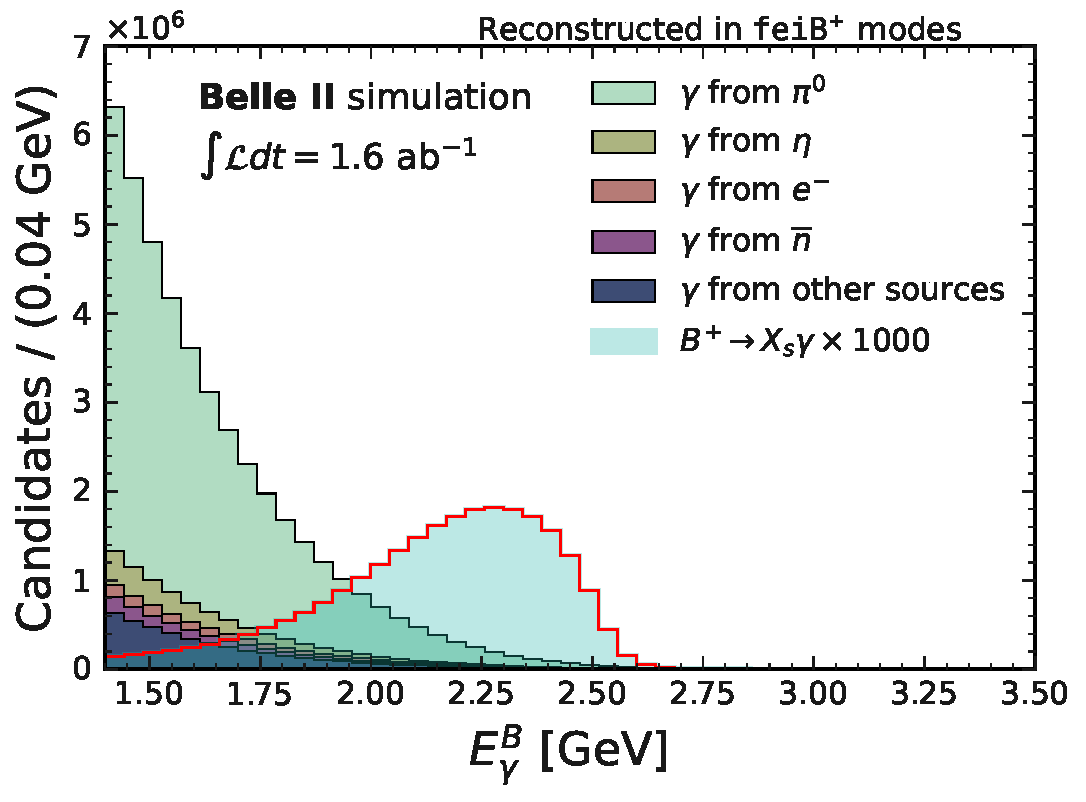
\includegraphics[width=0.45\textwidth]{figures/event_selection/Bp_photon_sources.pdf}
    }
    \subcaptionbox{\label{fig:bz_photon_sources}}{
        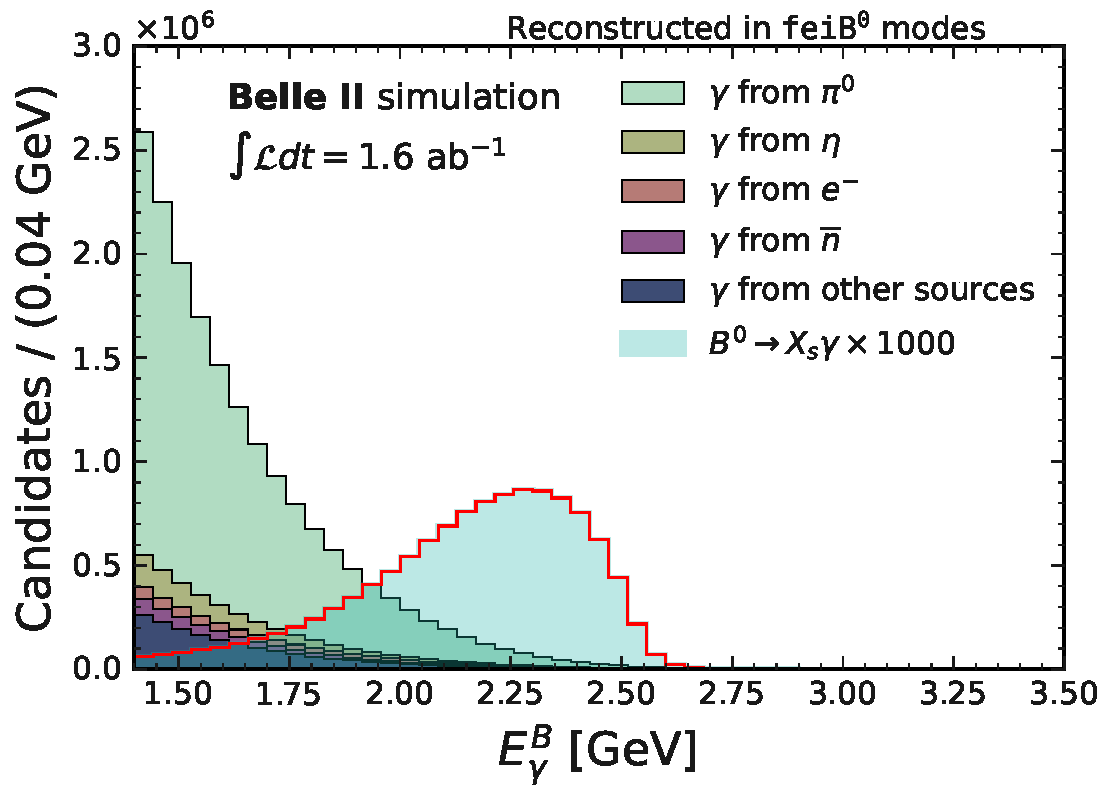
\includegraphics[width=0.45\textwidth]{figures/event_selection/Bz_photon_sources.pdf}
        }
    \caption{\label{fig:photon_sources} The background photon distribution after reconstruction in \feiBp and \feiBz modes, stacked by the photon mother-particle species.
    A scaled \BtoXsgamma spectrum is also overlaid.
    Only one photon candidate per event is shown, but it may still be paired with multiple tag-side candidates.
    Roughly 85\% of candidates originate in $\piz\ra\g\g$ or $\eta\ra\g\g$ decays.
    Other important backgrounds are photons from initial-state radiation, bremsstrahlung, and neutron-annihilation processes.
    These account for approximately 3\% each.
    The leftover 10\% originate in various other decays.}
\end{figure}

At this stage, \BtoXsgamma events make up 0.05\% of the \feiBp sample and 0.07\% of the \feiBz sample.
To reduce the discussed background components the following strategy is adopted:
\begin{itemize}
    \item Suppress misidentified photons (different particle species);
    \item Suppress $\piz\ra\g\g$ and $\eta\ra\g\g$ decays;
    \item Suppress \epem\ra\qqbar events;
    \item Reoptimise all selections simultaneously to adopt a final set of selections.
\end{itemize}

\subsection{Misidentified photon suppression}\label{sec:selection_clusZMVA}

Neutrons, $K_L^0$, protons, electrons and other charged hadrons where tracking for the particle did not succeed may leave clusters in the \ECL which are misidentified as photons.
The photon misidentification rate is given in \Cref{tab:misidentified_photons}.
The main misidentified photon candidates originate from neutrons with a small contribution from electron and $K_L^0$ showers.

\begin{table}[htbp!]
    \centering
    \caption{\label{tab:misidentified_photons} Photon misidentification rates after reconstruction.
    The majority of photons are identified correctly, with the largest component coming from misidentified neutron showers and $K_L^0$ deposits.
    The rates are similar for \feiBp and \feiBz modes which is consistent with the fact that this property is independent of the decaying $B$ charge.}
    \resizebox{1\textwidth}{!}{
\begin{tabular}{|l||c|c|c|c|c|c|c|c|c|c|c|}
    \hline
    Particle species & \multicolumn{2}{c|}{$\gamma$} & \multicolumn{2}{c|}{$n^0$} & \multicolumn{2}{c|}{$\en$} & \multicolumn{2}{c|}{$K_L^0$} & \multicolumn{2}{c|}{$p^-$} & Other \\
    \hline
    Candidate rate (\FEI \Bp | \Bz) & 96.1\% & 96.0\% & 2.4\% & 2.5\% & 0.5\% & 0.5\% & 0.5\% & 0.5\%  & 0.3\% & 0.3\% & 0.2\% \\
    \hline
\end{tabular}
}
\end{table}

The interactions of these particle species in the \ECL shower -- produce a cascade of secondary particles which may produce tertiary particles etc.
Generally, the total energy deposit and distribution between \ECL crystals, also known as \textit{shower-shape}, is different depending on the particle species due to their different radiation lengths.
This can be used to distinguish photon clusters using \MVA methods.
A technique achieving this, which uses the moments of Zernike polynomials, is documented in Ref.~\cite{Hershenhorn:2468}.
This approach is implemented in \basftwo and used in this analysis.
Here, a condensed overview of the approach is provided.

A complete set of complex two-dimensional polynomials is defined as:
\begin{equation}
    V_{nm}(\rho\cos\alpha,\rho\sin\alpha) = R_{nm}(\rho)e^{im\alpha},
\end{equation}
where ${x=\rho\cos\alpha, y=\rho\sin\alpha}$ are polar coordinates, $m$ is an integer and $R_{nm}(\rho)=V(\rho,0)$ is a polynomial of degree $n$.
The expression for a Zernike polynomial is given as:
\begin{equation}
    R_{nm}(\rho) = \sum^{\frac{n-|m|}{2}}_{s=0}(-1)^s \frac{(n-s)!}{ s! \left(\frac{n+|m|}{2}-s \right) ! \left( \frac{n-|m|}{2}-s\right) !}\rho^{n-2s}.
\end{equation}
The moments of a function $f(\rho\cos\alpha,\rho\sin\alpha)$ are expressed in terms of $V_{nm}$ as:
\begin{equation}
    Z_{nm} = \frac{n+1}{\pi} \int_0^{2\pi}\int^1_0 V^*_{nm}(\rho\cos\alpha,\rho\sin\alpha)f(\rho\cos\alpha, \rho\sin\alpha)\rho d\rho d\alpha.
\end{equation}
$Z_{nm}$ are called Zernike moments.
They have many useful properties that make them usable in image recognition, the field of optics, and more importantly, particle identification algorithms (see. Ref.~\cite{Hershenhorn:2468} and references therein).

A Dirac comb is defined to parametrise a particle shower in the \ECL as:
\begin{equation}
    f(\vec{x}) = \sum_i \delta(\vec{x}-\vec{x}_i)\frac{w_iE_i}{\sum w_iE_i},
\end{equation}
where $\vec{x}$ is a dimensionless crystal position in the perpendicular plane, $i$ is a crystal index, summing over all crystals in a given particle shower, and $E_i$ is the energy of the $i$-th crystal.
As showers can overlap, $w_i$ is the fraction of energy in a crystal that is associated with the currently investigated shower.
It can be shown, that Zernike moments for \ECL showers can then be expressed as:
\begin{equation}
    |Z_{nm}| = \frac{n+1}{\pi}\frac{1}{\sum_iw_iE_i}\left|\sum_iR_{nm}(\rho_i)e^{-im\alpha_i}w_iE_i\right|.
\end{equation}

The work in Ref.~\cite{Hershenhorn:2468} selects the best combination of eleven $|Z_{nm}|$ which provides the strongest separation between hadronic showers and electromagnetic showers.
The chosen combination of $|Z_{nm}|$ is combined using a \BDT and produces a single output, hereafter referred to as $\ZMVA\in(0,1)$.
The \ZMVA distributions for \BtoXsgamma candidates in generic \MC and signal \MC events are shown in \Cref{fig:zmva_distribution}.

\begin{figure}[htbp!]
    \centering
    \subcaptionbox{\label{fig:bp_zmva_distribution}}{
        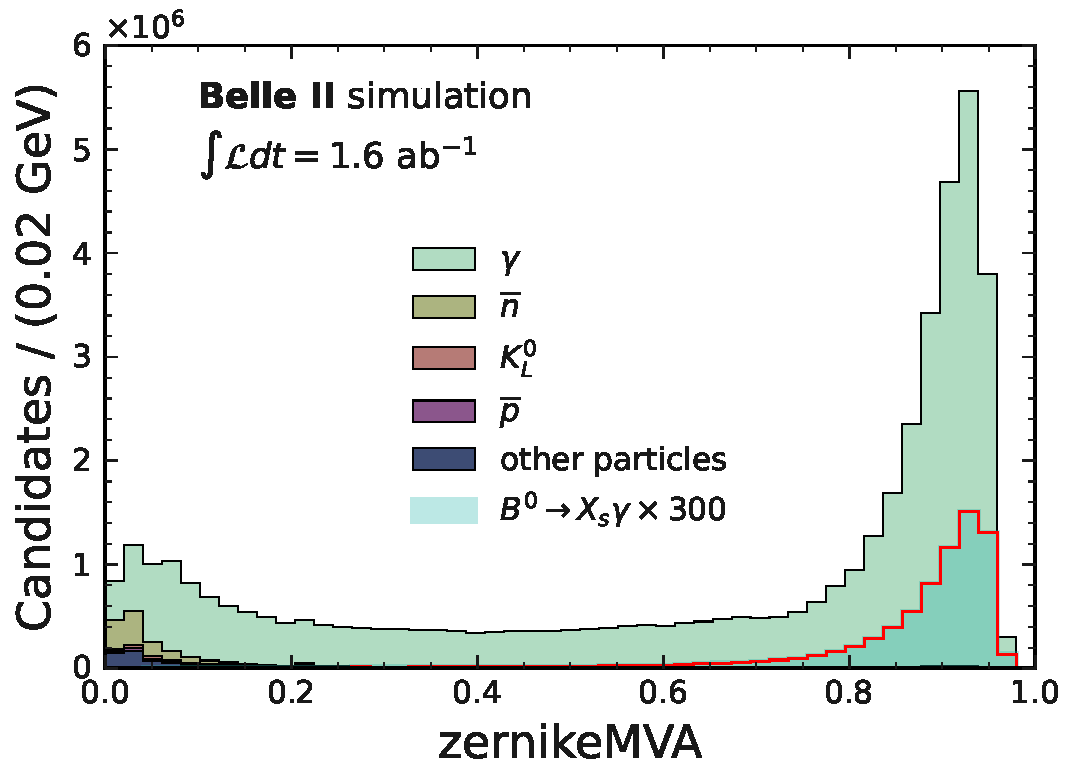
\includegraphics[width=0.45\textwidth]{figures/event_selection/Bp_zernikeMVA_mcPDG.pdf}
    }
    \subcaptionbox{\label{fig:bz_zmva_distribution}}{
        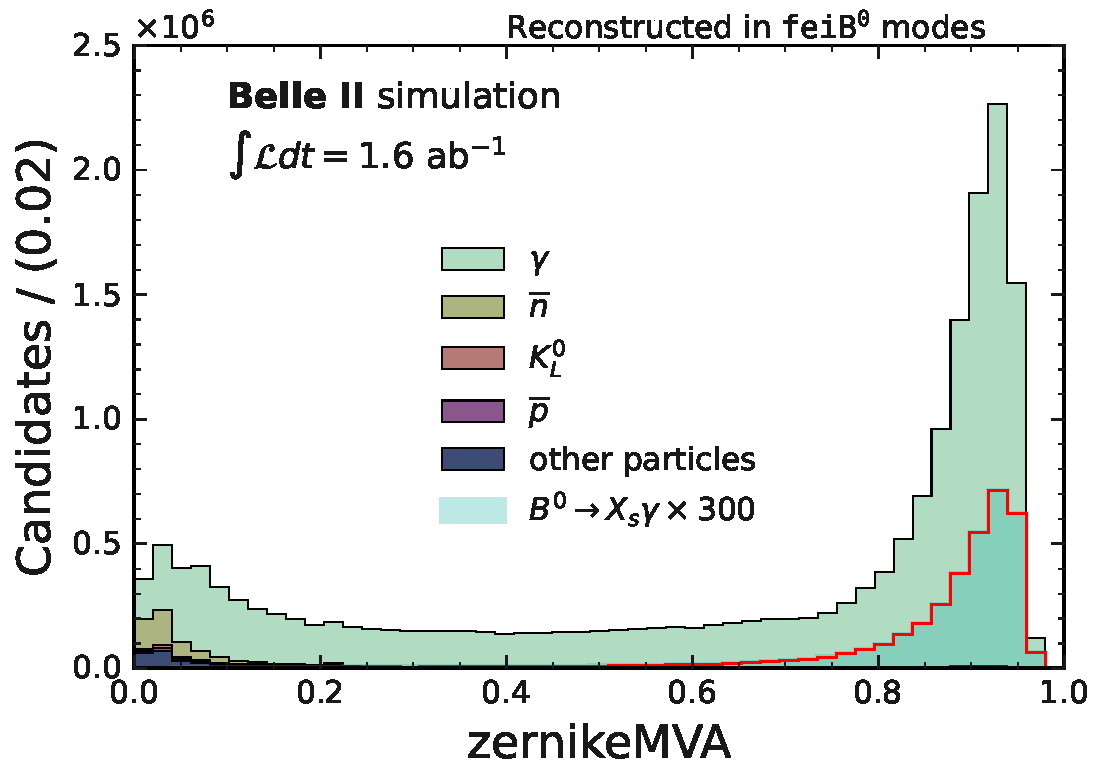
\includegraphics[width=0.45\textwidth]{figures/event_selection/Bz_zernikeMVA_mcPDG.pdf}
        }
    \caption{\label{fig:zmva_distribution} The distributions of the \ZMVA for different particle species that are reconstructed as photon candidates in \feiBp and \feiBz modes.
    The candidates presented in these Figures are the same as those in \Cref{fig:photon_sources}.
    A scaled \ZMVA distribution for \BtoXsgamma events is overlaid.
    A good separation is observed between real photons and hadronic showers misidentified as photons.}
\end{figure}

Overall, for true photons this distribution is strongly peaking in the $0.8-1$ region.
Misidentified hadrons peak close to 0.
For non-\BtoXsgamma photon candidates, this distribution remains relatively uniform in the $0-0.8$ region.
Moreover, \ZMVA provides a good separation against real photon candidates that originate in neutron annihilation events.
This is shown by a \ZMVA distribution exclusively for true photon candidates in \Cref{fig:zmva_distribution_sources}.

\begin{figure}[htbp!]
    \centering
    \subcaptionbox{\label{fig:bp_zmva_distribution_sources}}{
        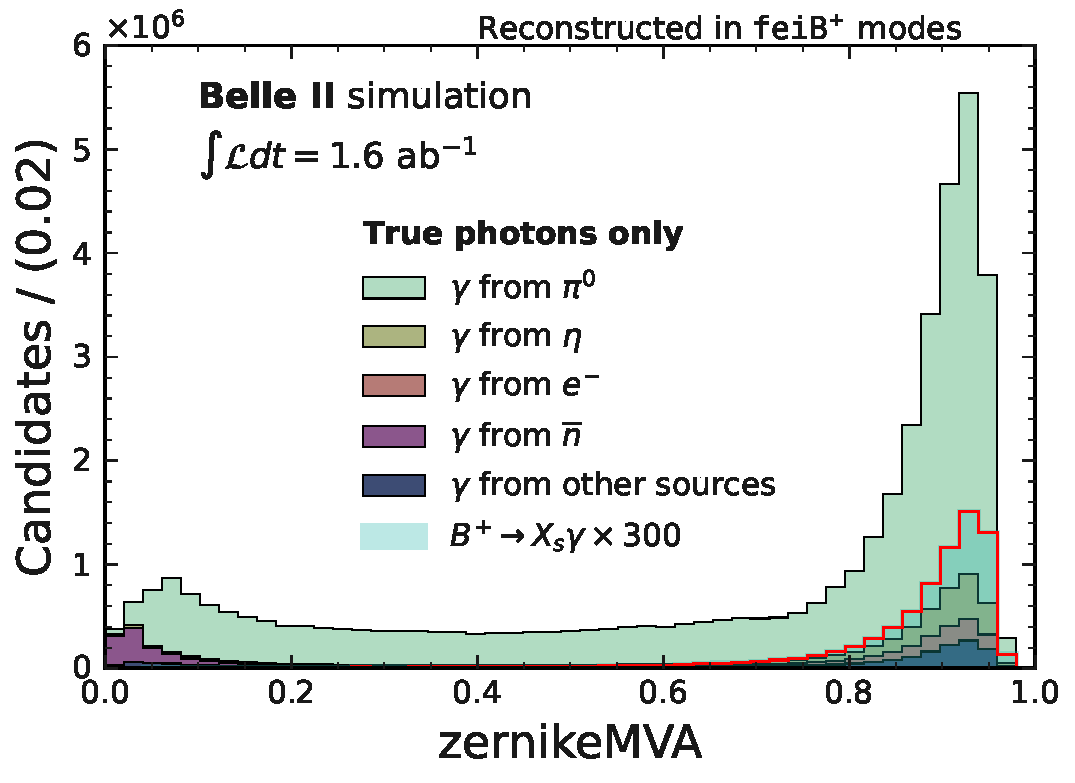
\includegraphics[width=0.45\textwidth]{figures/event_selection/Bp_zernikeMVA_true_photons_only.pdf}
    }
    \subcaptionbox{\label{fig:bz_zmva_distribution_sources}}{
        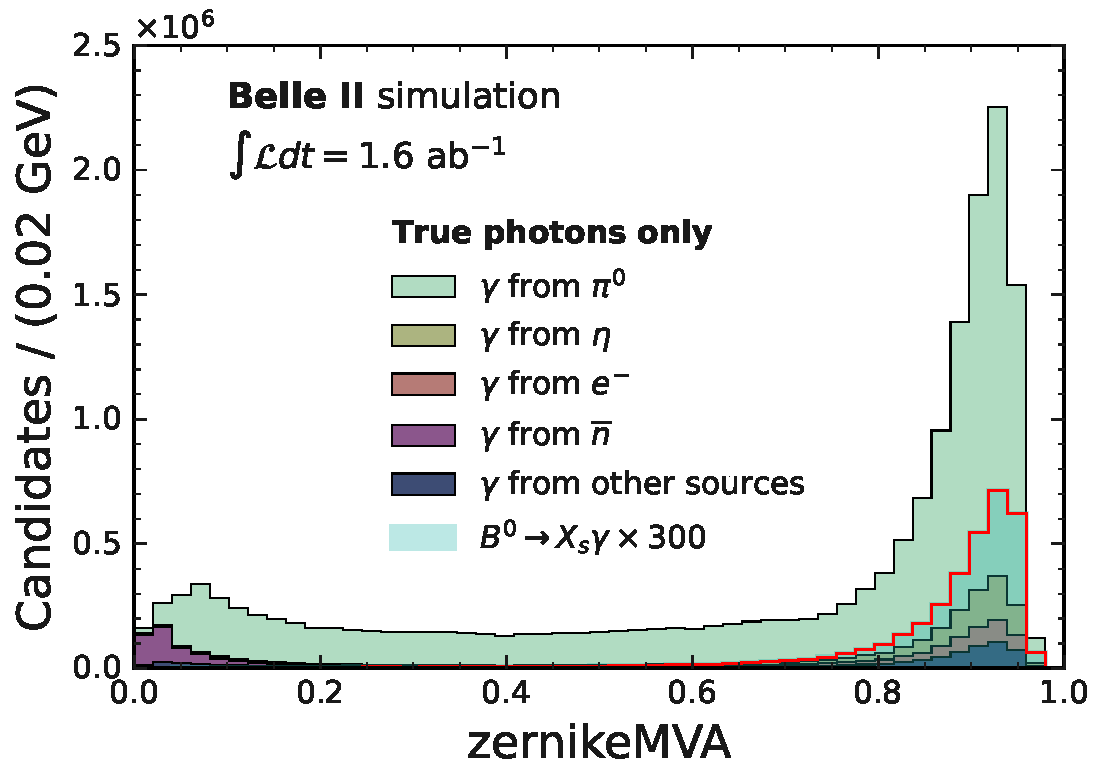
\includegraphics[width=0.45\textwidth]{figures/event_selection/Bz_zernikeMVA_true_photons_only.pdf}
        }
    \caption{\label{fig:zmva_distribution_sources} The distributions of the \ZMVA for different photon sources in generic \MC reconstructed in \feiBp and \feiBz modes.
    The candidates presented here are only those which are true photons in \Cref{fig:zmva_distribution}.
    A scaled \ZMVA distribution for \BtoXsgamma events is overlaid.
    Photons associated with neutron annihilation events are separated.}
\end{figure}

\subsection{Suppression of \texorpdfstring{\piz}{pi0} and \texorpdfstring{\eta}{eta} diphoton decays}\label{sec:selection_vetos}

85\% of background photons in this analysis originate from photons that are produced in $\piz\ra\g\g$ or $\eta\ra\g\g$ decays.
A lot of such light mesons originate in continuum events, but they are prominent even in \BB events.
Therefore, an efficient mechanism to suppress \piz- and $\eta$-related photon candidates is required.

In this analysis, a suppression tool, called \textit{\piz~and~\eta~veto} is utilised.
It is implemented as part of \basftwo and is a standard Belle~II approach for suppressions of radiative backgrounds from light mesons.
Here, an overview of the training and the validation process is provided which is performed by an independent analysis.

The general idea of the \piz~and~\eta~veto is to pair the high energy photon signal candidate (\textit{hard} photon) with lower energy photons (\textit{soft} photons) in the event.
The compatibility of the combination with a $\piz\ra\g\g$ or $\eta\ra\g\g$ decay is evaluated and a probability-like quantity is calculated to quantify it.

The soft photon candidate is selected with an energy of $30~\mev$ ($40~\mev$ in the backward \ECL endcap) for $\piz$ or $60~\mev$ for $\eta$.
The photon is also required to have deposited the energy in 2 or more crystals.
Furthermore, photon candidates are required to have an associated cluster time less than one standard deviation away from 0.
These selections ensure that beam background photons, neutral hadrons misidentified as photons and misreconstructed charged particles are not included in the soft photon sample.

The soft photons that pass these selections are combined with the hard photon candidate.
The following observables are then calculated and used to train a \MVA classifier:
\begin{itemize}
    \item Invariant mass of the soft photon and hard photon combination;
    \item Soft photon energy in the laboratory frame;
    \item Soft photon \ECL cluster polar angle;
    \item Distance between the soft photon \ECL cluster and the nearest track extrapolated to the \ECL;
    \item Helicity angle of the combination.
\end{itemize}
The classifier for $\eta\ra\g\g$ includes additional observables to increase the separation power:
\begin{itemize}
    \item \ZMVA of the soft photon;
    \item Number of crystals where the soft photon has deposited energy;
    \item Ratio of soft photon energy in 3-by-3 crystals around the central crystal to soft photon energy in the 5-by-5 crystals with the corner crystals removed.
\end{itemize}
For every combination of a soft and hard photon, the \MVA produces an output between 0 and 1.
The same hard photon is paired with all soft photons in a given event, and the largest \MVA output is assigned to it as the $\piz$ or $\eta$ probability.
This \MVA output is denoted as \piVeto or \etaVeto, respectively.
Note that despite the nomenclature, this variable is only probability-like (i.e. $\mathcal{P}\in(0,1)$) but does not truly represent a probability.
The distributions for \piVeto and \etaVeto are shown in \Cref{fig:vetos}.
In all cases, \BtoXsgamma can be seen to be strongly peaking near 0, consistent with photons that do not originate from light unflavoured meson decays.

\begin{figure}[htbp!]
    \centering
    \subcaptionbox{\label{fig:bp_piveto}}{
        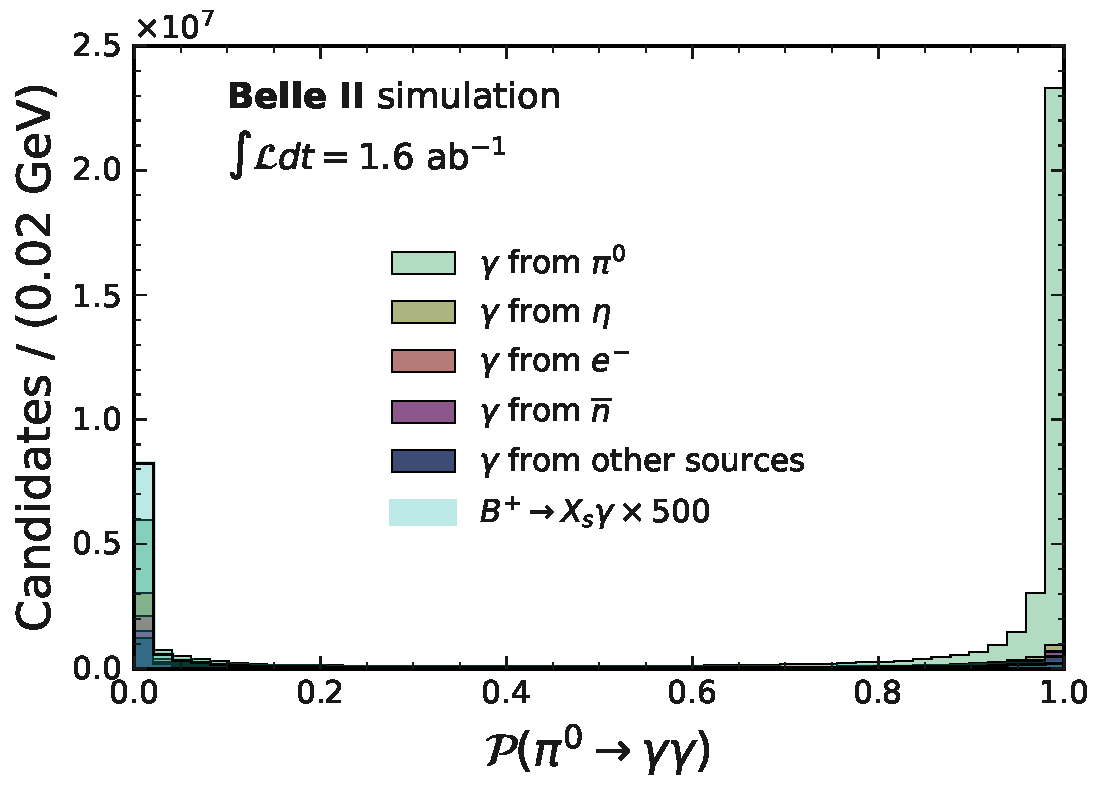
\includegraphics[width=0.45\textwidth]{figures/event_selection/Bp_piVeto.pdf}
        }
    \subcaptionbox{\label{fig:bz_piveto}}{
        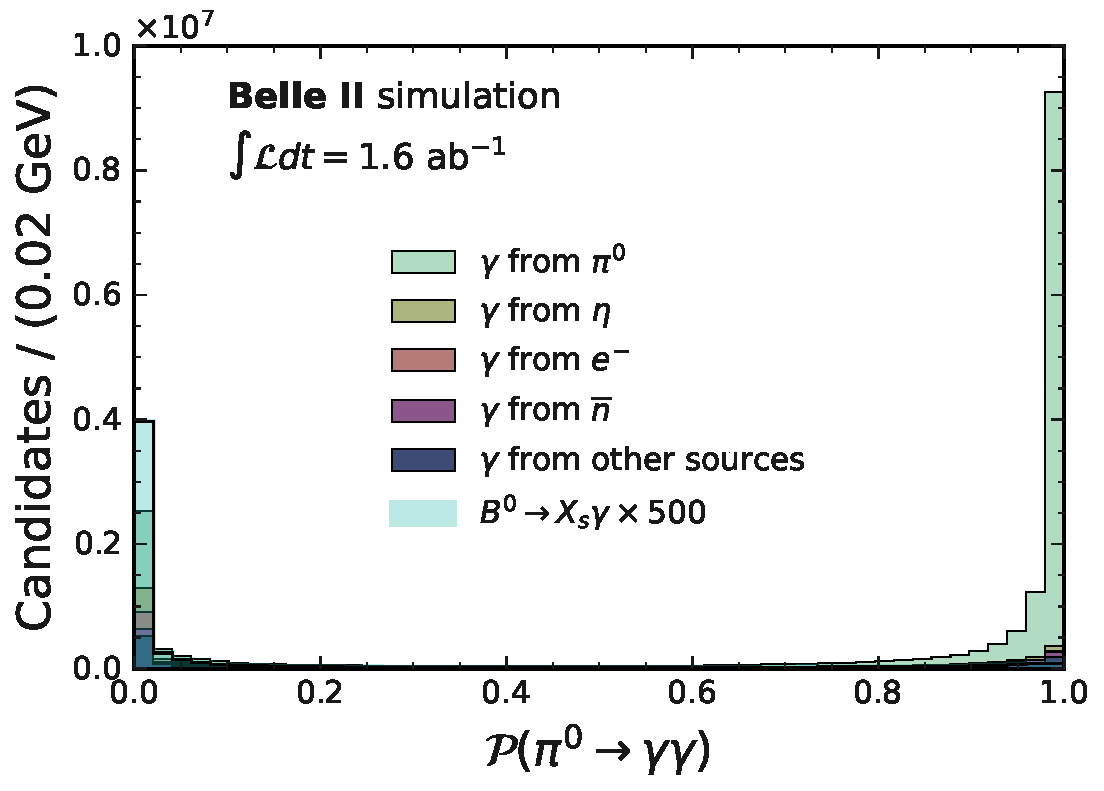
\includegraphics[width=0.45\textwidth]{figures/event_selection/Bz_piVeto.pdf}
        }
    \subcaptionbox{\label{fig:bp_etaveto}}{
            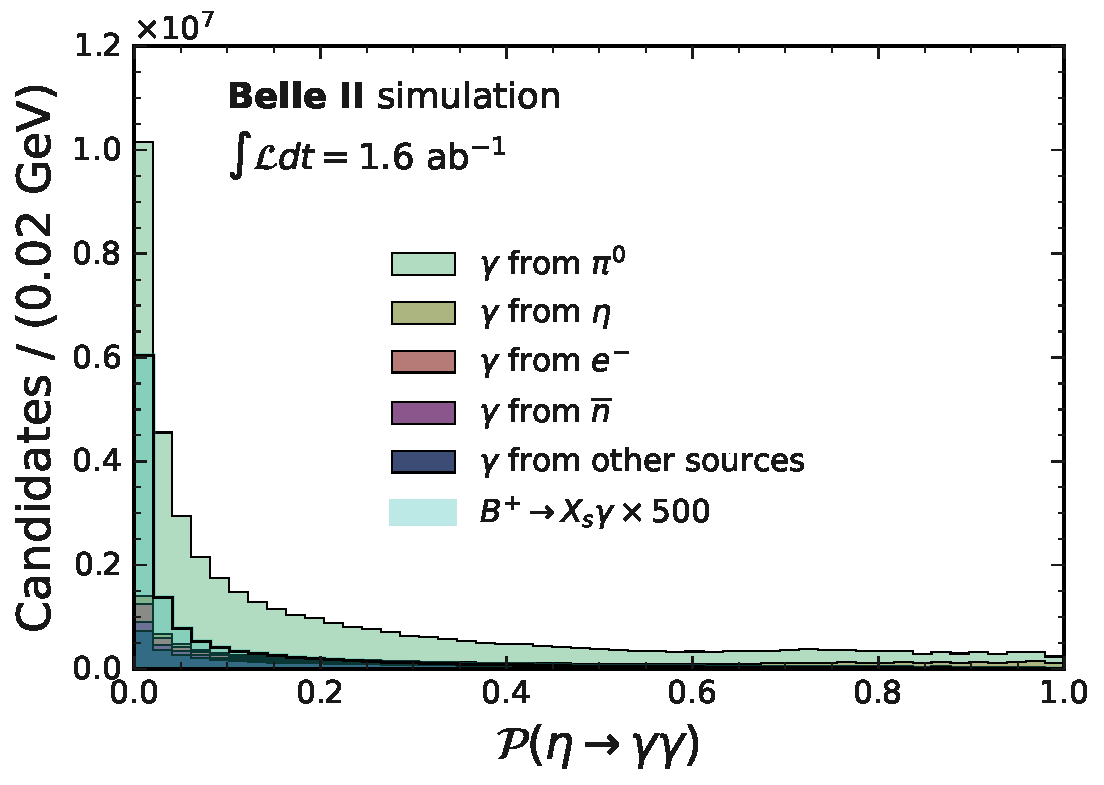
\includegraphics[width=0.45\textwidth]{figures/event_selection/Bp_etaVeto.pdf}
        }
    \subcaptionbox{\label{fig:bz_etaveto}}{
            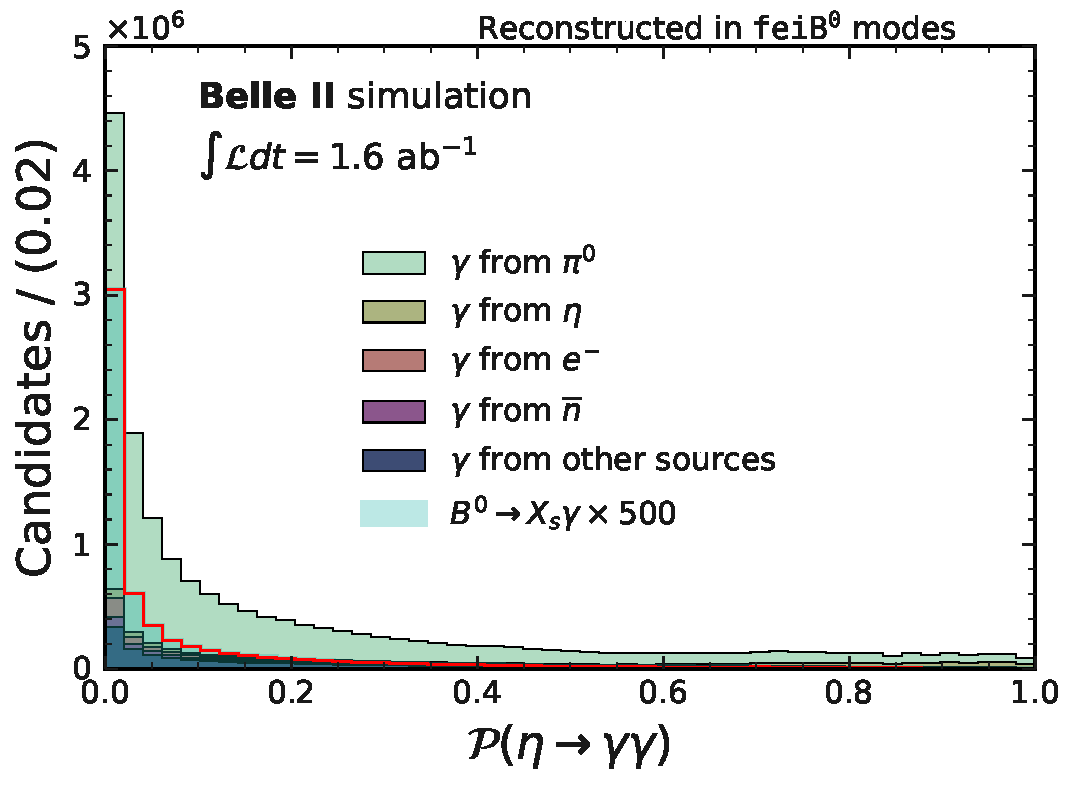
\includegraphics[width=0.45\textwidth]{figures/event_selection/Bz_etaVeto.pdf}
        }
    \caption{\label{fig:vetos} The distributions of \piVeto (\Cref{fig:bp_piveto,fig:bz_piveto}) and \etaVeto (\Cref{fig:bp_etaveto,fig:bz_etaveto}) 
    for different photon sources in generic \MC reconstructed in \feiBp and \feiBz modes.
    This is shown for all photon candidates included in \Cref{fig:photon_sources}.
    Scaled respective veto probability distributions for \BtoXsgamma events are overlaid.
    The separation power of \etaVeto is hidden by a large number of $\piz\ra\g\g$ events in \Cref{fig:bp_etaveto,fig:bz_etaveto}.
    It is apparent again when \piz decays events are removed from the sample as shown in \Cref{fig:vetos_nopi}.
    }
\end{figure}

For the case of \piz veto, shown in \Cref{fig:bp_piveto,fig:bz_piveto}, an excellent separation is observed between photons originating in \piz decays and other photons.
\BtoXsgamma and other non-\piz photon candidates also show a small peak at high-\piVeto values, which alludes to a small inefficiency of the algorithm.
However, compared to the separation power provided, this is an acceptable trade-off.
For the \etaVeto, the separation is less clear.
The reason for this is the fact that the generic \MC sample is dominated by $\piz\ra\g\g$ decays which are not targeted by the \etaVeto classifier.
Removing $\piz\ra\g\g$ decays from the sample, a clear separation of photon candidates originating in $\eta$ decays from other types of decays becomes apparent (see \Cref{fig:vetos_nopi}).

\begin{figure}[htbp!]
    \centering
    \subcaptionbox{\label{fig:bp_etaveto_nopi}}{
            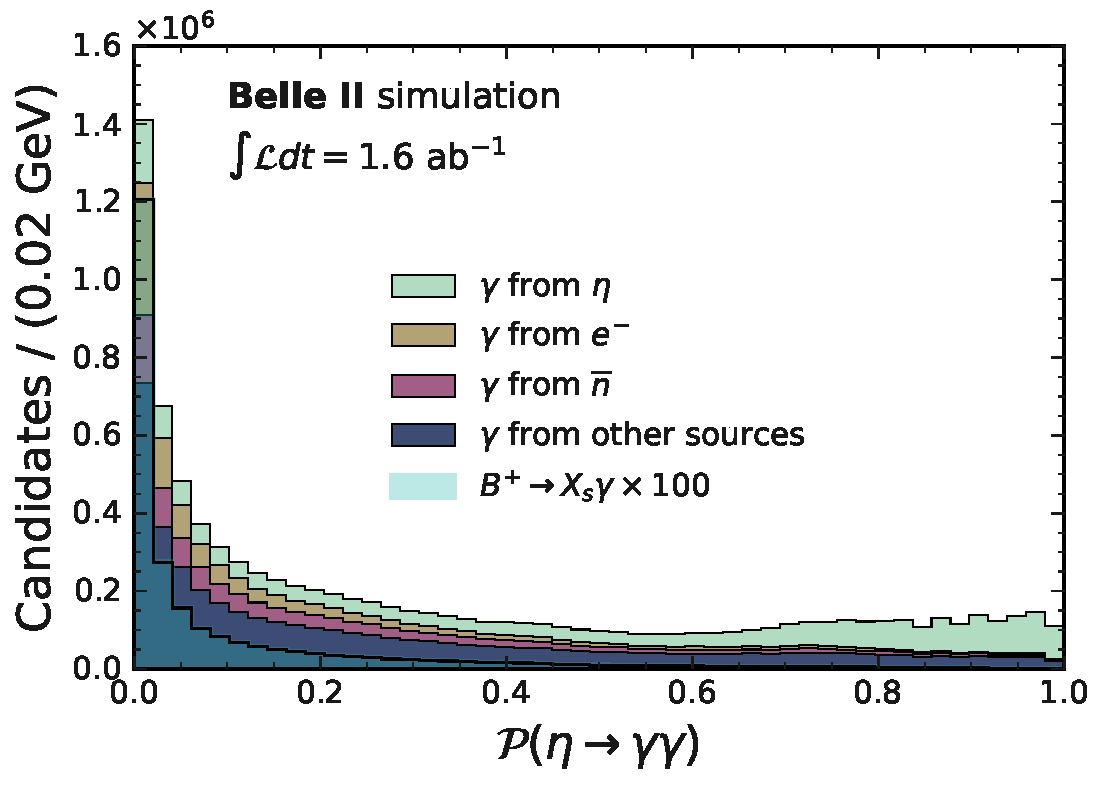
\includegraphics[width=0.45\textwidth]{figures/event_selection/Bp_etaVeto_nopi.pdf}
        }
    \subcaptionbox{\label{fig:bz_etaveto_nopi}}{
            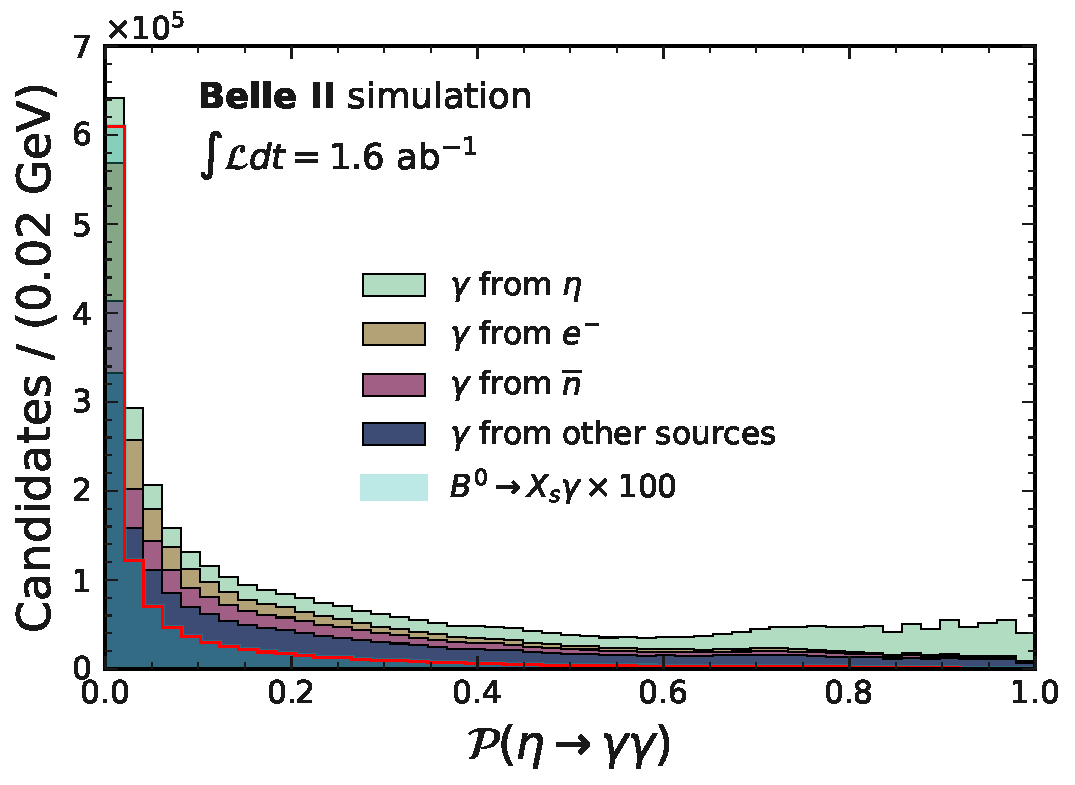
\includegraphics[width=0.45\textwidth]{figures/event_selection/Bz_etaVeto_nopi.pdf}
        }
    \caption{\label{fig:vetos_nopi} The distributions of \etaVeto
    for different photon sources in generic \MC reconstructed in \feiBp and \feiBz, but with photons that are associated with $\piz\ra\g\g$ removed.
    This is equivalent to \Cref{fig:bp_etaveto,fig:bz_etaveto} with the \piz component not included.
    A scaled \etaVeto distribution for \BtoXsgamma events is overlaid.
    Although the separation power is not as strong as in the case of \piVeto (\Cref{fig:bp_piveto,fig:bz_piveto}), a clear peak at low-\etaVeto can be seen for \BtoXsgamma.
    }
\end{figure}

\subsection{Signal-photon background suppression correlation}\label{sec:signal_photon_correlation}

Even though no direct selection is applied on the $X_s$ system, through direct or higher-order correlations with \EB, a bias may be introduced to the photon energy.
To ensure that no such correlation is introduced, a correlation study is performed for \piVeto, \etaVeto and \ZMVA observables.
In principle, it is acceptable if the selection introduces a bias to the background -- as long as this bias is well reproduced in simulation.
The latter will be validated in \Cref{sec:corrections,sec:signal_modelling}.
Therefore, the study is performed exclusively focusing on \BtoXsgamma events, as it is aimed to ensure that the photon energy spectrum itself is minimally biased.

\begin{figure}[htbp!]
    \centering
    \subcaptionbox{\label{fig:bp_zmva_correlation}}{
            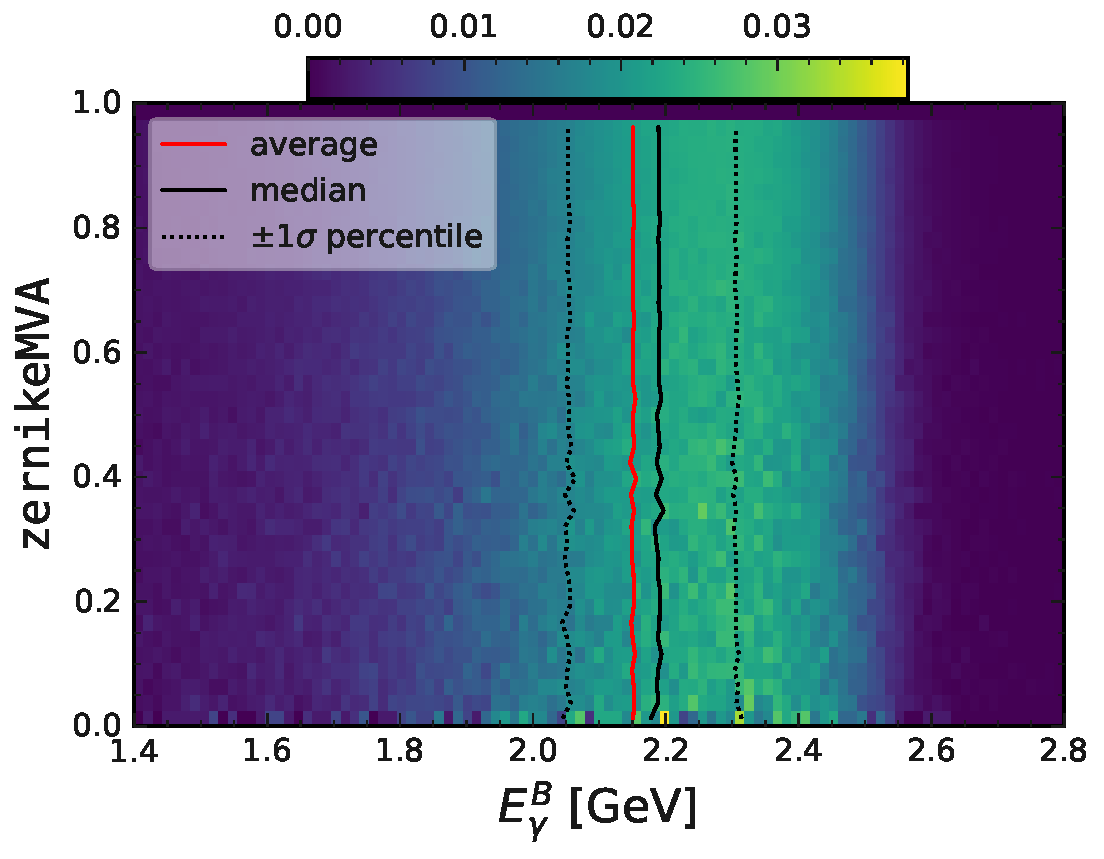
\includegraphics[width=0.31\textwidth]{figures/event_selection/Bp_zernikeMVA_correlation.pdf}
        }
    \subcaptionbox{\label{fig:bp_piveto_correlation}}{
            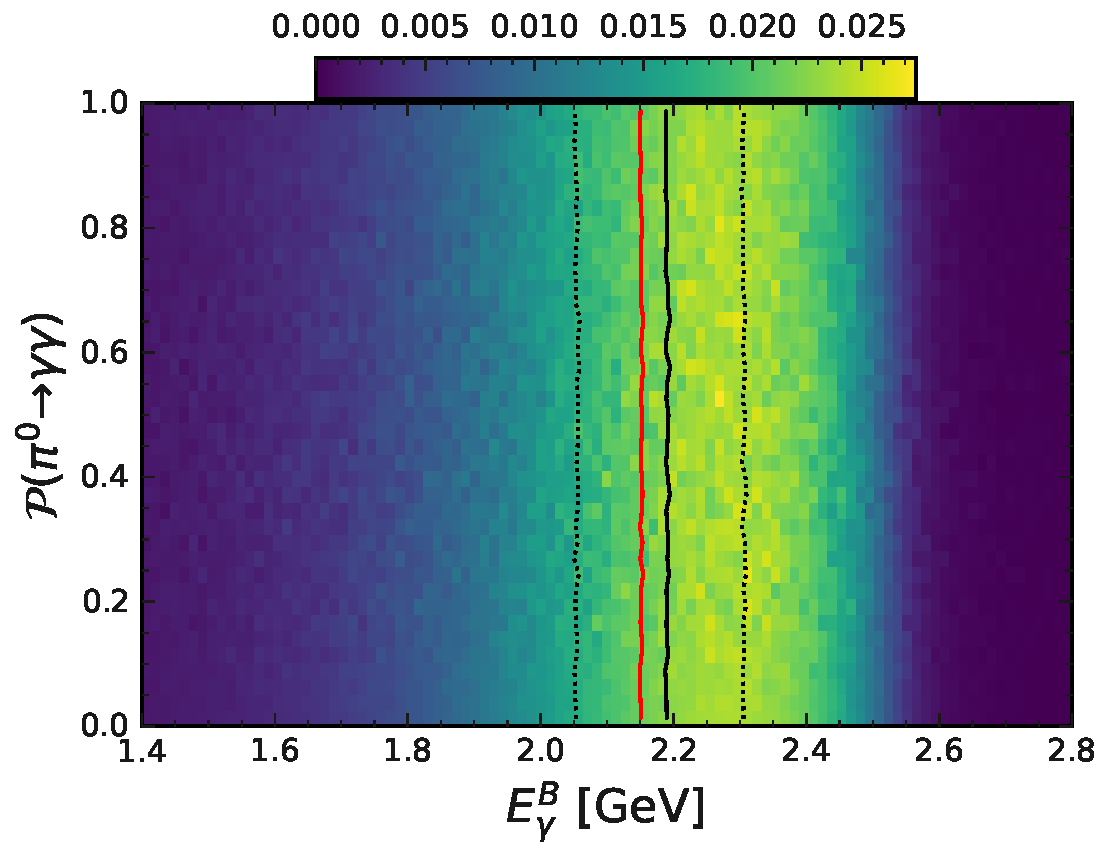
\includegraphics[width=0.31\textwidth]{figures/event_selection/Bp_piVeto_correlation.pdf}
        }
    \subcaptionbox{\label{fig:bp_etaveto_correlation}}{
            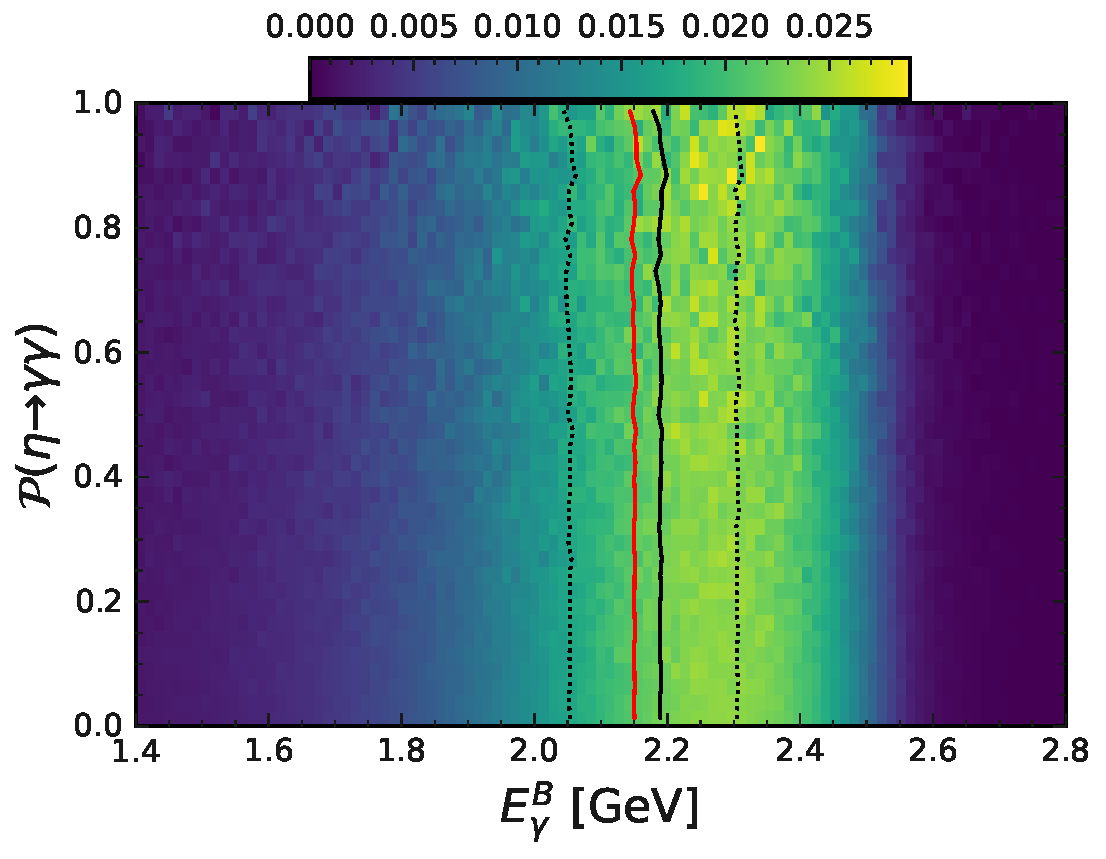
\includegraphics[width=0.31\textwidth]{figures/event_selection/Bp_etaVeto_correlation.pdf}
        }
    \subcaptionbox{\label{fig:bz_zmva_correlation}}{
            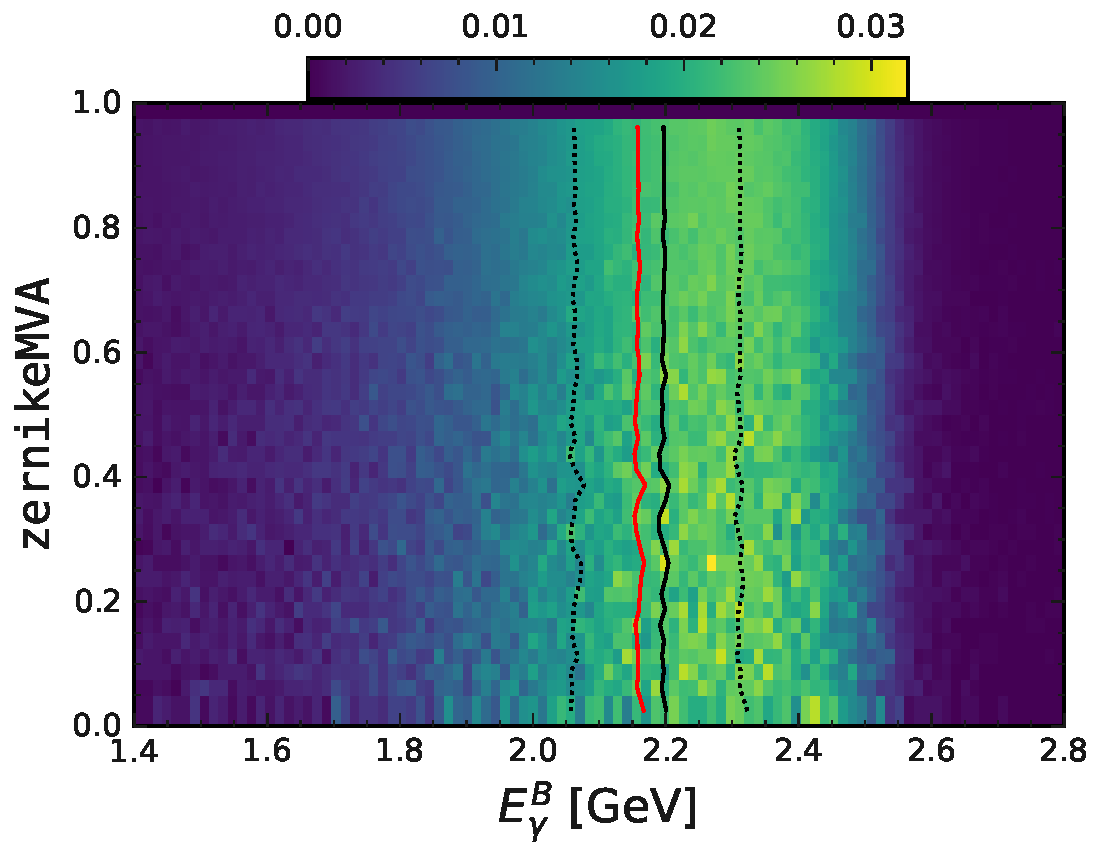
\includegraphics[width=0.31\textwidth]{figures/event_selection/Bz_zernikeMVA_correlation.pdf}
        }
    \subcaptionbox{\label{fig:bz_piveto_correlation}}{
            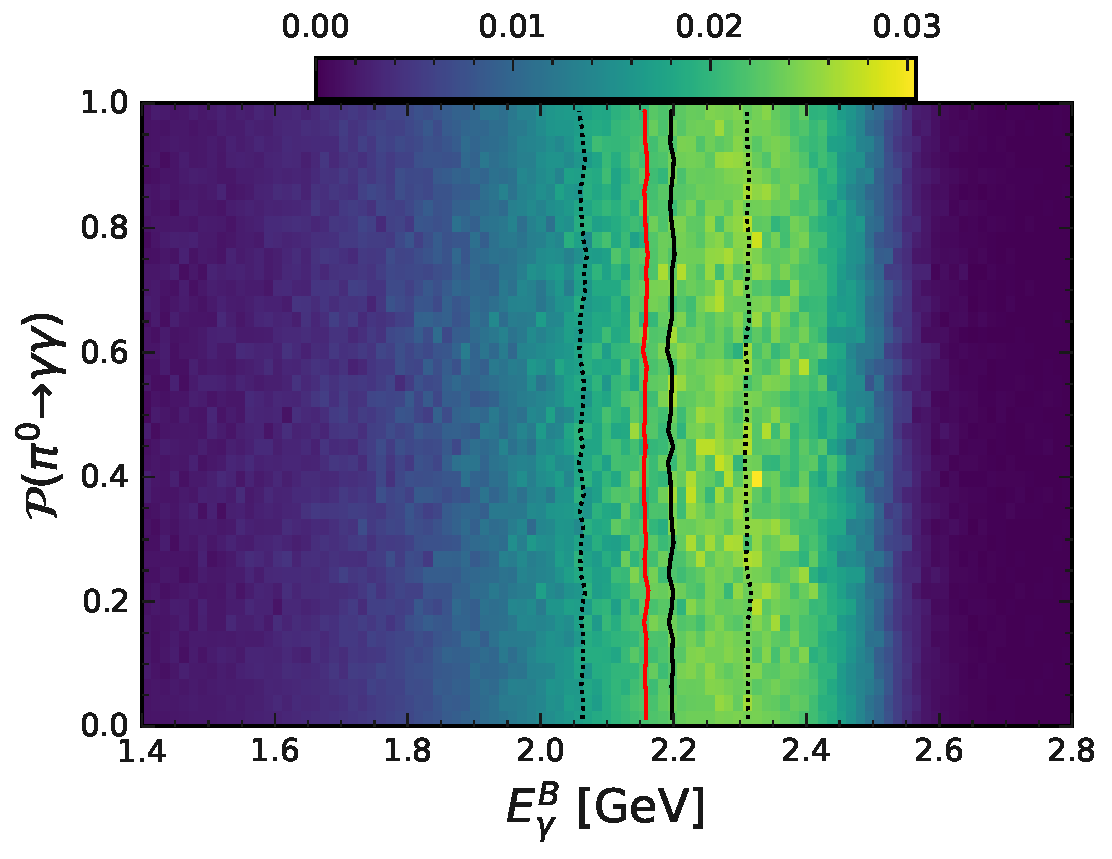
\includegraphics[width=0.31\textwidth]{figures/event_selection/Bz_piVeto_correlation.pdf}
        }
    \subcaptionbox{\label{fig:bz_etaveto_correlation}}{
            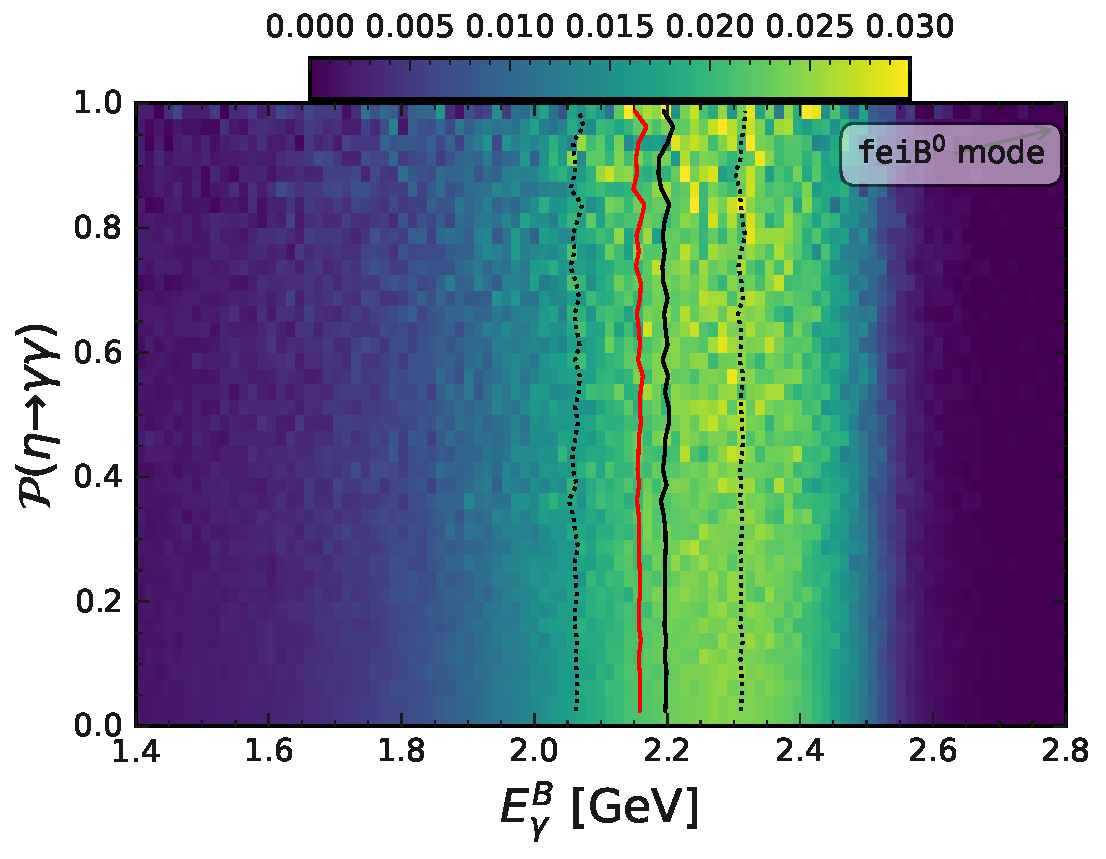
\includegraphics[width=0.31\textwidth]{figures/event_selection/Bz_etaVeto_correlation.pdf}
        }
    \caption{\label{fig:selection_correlations} Correlation tests for background suppression observables described in \Cref{sec:photon_selection}, depicted as a 2D histogram.
    Each row is normalised such that all bins within that row add up to 1.
    For signal \BptoXsgamma events, the tests are shown
    in \Cref{fig:bp_zmva_correlation,fig:bp_piveto_correlation,fig:bp_etaveto_correlation},
    and for \BztoXsgamma in \Cref{fig:bz_zmva_correlation,fig:bz_piveto_correlation,fig:bz_etaveto_correlation}.
    All figures share the same legend provided in \Cref{fig:bp_zmva_correlation}.
    In the red line, the average photon energy, $\expval{\EB}$, is shown as a function of the tested observable.
    In black and black-dotted lines: median and $\pm 1 \sigma$ percentile values of \EB, respectively.
    No strong dependence can be observed in any of the quantities or the 2D maps.
    }
\end{figure}

A two-dimensional map of ${\piVeto,\etaVeto,\ZMVA}$ versus \EB is given in \Cref{fig:selection_correlations}.
Because the distributions of the three variables used for background suppression are not uniform, each row is normalised such that the sum of each row is equal to unity.
This makes the comparison between differently populated bins simpler.
The Figure also denotes the average, the median and $\pm 1\sigma$ percentiles of \EB.
No strong bias is introduced by any of the observables to any of these quantities.
Furthermore, the structure itself remains constant across all bins and no clear dependence on \EB can be seen.
No significant differences between different \FEI modes are observed.
It is therefore concluded that the selections are unbiasing and suitable for signal-side photon background suppression.
The exact selections on these observables are optimised simultaneously with continuum event suppression in \Cref{sec:final_optimisation}.